%%%%%%%%%%%%%%%%%%%%%%%%%%%%%%%%%%%%%%%%%%%%%%%%%%%%%%%%%%%%%%%%%%%%%%
%     File: ExtendedAbstract_intro.tex                               %
%     Tex Master: ExtendedAbstract.tex                               %
%                                                                    %
%     Author: Andre Calado Marta                                     %
%     Last modified : 27 Dez 2011                                    %
%%%%%%%%%%%%%%%%%%%%%%%%%%%%%%%%%%%%%%%%%%%%%%%%%%%%%%%%%%%%%%%%%%%%%%
% State the objectives of the work and provide an adequate background,
% avoiding a detailed literature survey or a summary of the results.
%%%%%%%%%%%%%%%%%%%%%%%%%%%%%%%%%%%%%%%%%%%%%%%%%%%%%%%%%%%%%%%%%%%%%%

\section{Introduction and motivation}
\label{sec:intro}

%- Higgs pair production as a benchmark physics process for HL and future colliders (discovery inaccessible at the LHC)\\
%- Boosted analysis shows better sensitivity because QCD background can be kept under control \\
%- When using boosted jets we need to resolve their substructure (jet substructure observables)\\
%- The granularity of the (hadronic) calorimeter is a key parameter that determines how well we can resolve the substructure \\
%- The final state with four b quarks benefits from the largest BR and is a source of fully hadronic boosted Higgs jets \\
%- Goals of the work: estimate analysis sensitivity to Higgs trilinear coupling and study the influence of the HCAL granularity in the analysis \\

A lot of work is currently being put into designing and understanding the physics reach of future particle colliders. The hadronic Future Circular Collider (FCC-hh) study, led by CERN, is one of the possibilities that is currently being analyzed. Its baseline design consists of a $100$ km ring located in the Geneva area capable of delivering proton-proton collisions at a center of mass energy of $100$ TeV. The next milestone for this project is the delivery of a Conceptual Design Report (CDR) by the end of 2018. This document should include a first cost estimate as well as a compilation of preliminary analysis that illustrate the physics potential of such an accelerator.

A particularly interesting benchmark process to be studied in future colliders is the production of pairs of Higgs bosons (or di-Higgs production). This process is sensitive to the value of the Higgs boson triple coupling that determines the shape of the Higgs potential and therefore plays a crucial role in the electroweak symmetry breaking mechanism. The leading order Feynamn diagrams that contribute to Higgs pair production through gluon-gluon fusion are shown in figure \ref{fig:hh_diag}. The top diagram is the one that provides sensitivity to the triple coupling.

\begin{figure}[h]
	\centering
	\feynmandiagram [baseline=(current bounding box.center),small, horizontal=e to f] {
		a -- [gluon, edge label'=\(g\)] b -- [anti fermion] c -- [gluon, edge label'=\(g\)] d,
		b -- [fermion] e -- [fermion] c,
		e -- [scalar, edge label'=\(h^*\)]  f,
		h -- [scalar, edge label'=\(h\)] f -- [scalar, edge label'=\(h\)] i,
		a -- [opacity=0] d,
	};\\
	\feynmandiagram[baseline=(current bounding box.center),small, layered layout,horizontal=a to b] {
		% Draw the top and bottom lines
		i1 -- [gluon, edge label'=\(g\)] a-- [anti fermion] b-- [scalar, edge label'=\(h\)] f1,
		i2 -- [gluon, edge label'=\(g\)] c-- [fermion] d-- [scalar, edge label'=\(h\)] f2,
		% Draw the two internal fermion lines
		{ [  same layer	] a -- [fermion] c },
		{ [  same layer] b -- [anti fermion] d},
	};
	\caption{Feynman diagrams for the $gg\rightarrow hh$ process at leading order.}
	\label{fig:hh_diag}
\end{figure}

However, searches for di-Higgs production are extremely challenging mainly because the cross section of this process is very small, of the order of tens of femtobarns (fb). Even with the entire dataset that is expected to be accumulated during the LHC's and its high luminosity upgrade lifetime ($O(3)~\text{ab}^{-1}$), it is very unlikely that we will be able to declare the observation of this process. Therefore, the discovery of di-Higgs production relies on future colliders making it a key benchmark process.

In this work we focus on the final state with four b quarks. The $h\rightarrow b\overline{b}$ decay has the largest of all Higgs branching ratios (BR), approximately $58\%$. Therefore this final state maximizes the cross section times branching of the $hh\rightarrow b\overline{b}b\overline{b}$ process. However, for this final state, the dominant background is multijet production through quantum chromodynamics (QCD) processes whose cross section is a lot larger than that of the signal. Nonetheless, it is a well known characteristic of QCD interactions that the partons (and jets) produced tend to have a low transverse momentum ($p_T$). This indicates that exploring a high $p_T$ region of the phase space could be the key to suppress the QCD multijet background. Such region is called boosted due to the high Lorentz boost of the objects involved. In this kinematic regime, traditional jet reconstruction algorithms, that establish a one to one correspondence between the partons and the jets, begin to fail because the $\Delta R=\sqrt{(\Delta\phi)^2+(\Delta\eta)^2}$ distance between the b quarks, $\Delta R(b\overline{b})$, gets increasingly smaller as the $p_T$ of the mother Higgs boson, $p_T(h_1)$, increases. This is shown in figure \ref{fig:deltaRbb_pt}. State of the art jet reconstruction techniques \cite{jetsub} use a single jet with a large $R$ parameter to reconstruct both b quarks as a single jet that is used as a $\textit{proxy}$ for the Higgs boson. In order to extract as much information as possible from these jets it is important to analyze its intrinsic structure, referred to as substructure. Such techniques are fairly recent and usually explore the existence of localized energy maximums inside a large $R$ jet (subjets). For example, a jet that contains the two b quarks coming from the decay of a Higgs boson is expected to be more compatible with the existence of two subjets than a jet produced by a QCD process.

\begin{figure}[h]
	\centering
	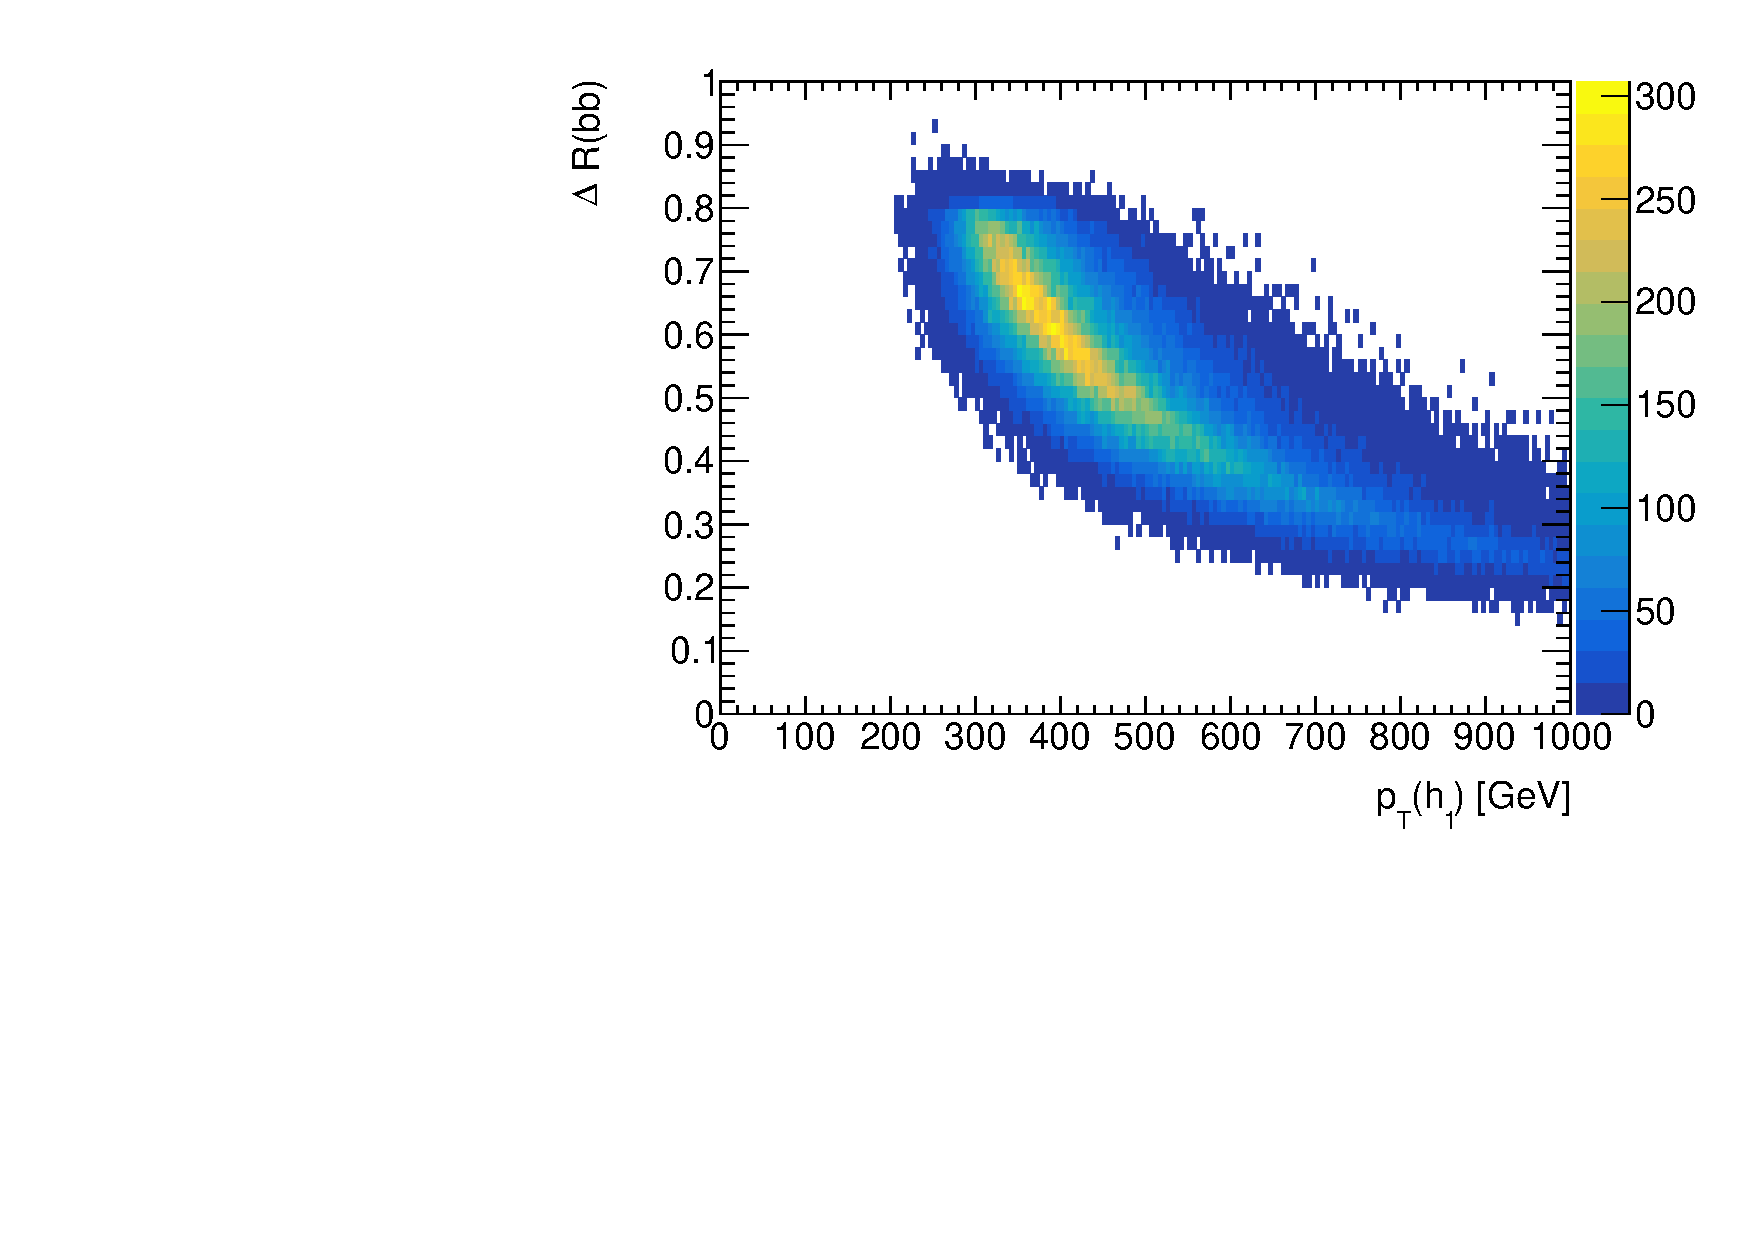
\includegraphics[trim={.5cm 0 0 0},clip,width=\linewidth]{./images/hist_deltaR_bb_pt.pdf}
	\caption{$\Delta R$ between the b quarks from the decya of the leading Higgs candidate as a function of its $p_T$.}
	\label{fig:deltaRbb_pt}
\end{figure}

From the point of view of detector design for the FCC-hh, as well as for future upgrades of existent detectors such as the ATLAS one, the granularity of the hadronic calorimeter (HCAL) is a key parameter because it greatly influences the ability of the detector to resolve the substructure of large $R$ jets. 

The main goal of this project is to use boosted di-Higgs production in the four b quarks final state to study the influence of the granularity of the HCAL in the significance ($S/\sqrt{B}$) that can be achieved.  
